\documentclass[12pt]{report}
\usepackage{setspace}  %use this package to set linespacing as desired
\usepackage{array}
\usepackage{graphicx}
\usepackage{subcaption}
\usepackage{amsmath}
\usepackage{color,soul}
\usepackage[counterclockwise, figuresleft]{rotating}

\begin{document}
\doublespacing

\clearpage
\chapter{Approach}

\section{Evaluation Metrics} \label{section:eval_metrics}

The efficacy of a shadow removal algorithm on a frame is evaluated with the popular metrics \textit{Detection} ($\eta$) and \textit{Discrimination} ($\xi$) (Eqn. \ref{eqn:detection}, Eqn. \ref{eqn:discrimination}) [\ref{to wherever they originated}]. These formulae measure how many shadow pixels are correctly identified, and how many foreground object pixels are correctly preserved, respectively. The metrics are calculated using true positives (TP) and false negatives (FN) of both foreground pixels and shadow pixels. Subscripts signify operations on shadow pixels ($S$) or foreground pixels ($F$).

\begin{equation}
\eta = \dfrac{TP_{S}}{TP_{S} + FN_{S}} \label{eqn:detection}
\end{equation}

\begin{equation}
\xi = \dfrac{TP_{F}}{TP_{F} + FN_{F}} \label{eqn:discrimination}
\end{equation}

\section{Shadow Removal Methods} \label{section:removalmethods}

Standardized implementations of popular shadow removal methods, including ground truths, backgrounds, and frames, are used courtesy of A. Sanin, C. Sanderson, B.C. Lovell (http://arma.sourceforge.net/shadows), licensed under GPL v3+ and written in C++.

\subsection{Chromacity}

\textit{Chromacity}, or \textit{hue}, represents the base color of a pixel, and is separable from brightness and saturation. Chromacity-based shadow removal methods maintain that a pixel, when covered by a shadow, loses luminosity (or brightness), while retaining its chromacity. This assumption is referred to as  color constancy, or linear attenuation. This study implements one such algorithm from Cucchiara et al. [\ref{gucciara}], implemented using the Hue-Saturation-Value (HSV) color representation. 

Cucchiara et al. observe a shadowed pixel in the foreground ($fg_{p}$) retains its hue when compared to the corresponding background pixel ($bg_{p}$), while losing saturation and intensity (value). In order to be considered a shadow, the hue, saturation, and value of $fg_{p}$ must fall within the pre-determined thresholds $\tau_{H}$, $\tau_{S}$, and [$\beta_{1}$, $\beta_{2}$] (Eqn. \ref{eqn:huethresh}, \ref{eqn:satthresh}, \ref{eqn:brightthresh}).

\begin{equation} \label{eqn:huethresh}
| fg_{p}(H) - bg_{p}(H) | \leq \tau_{H}
\end{equation}

\begin{equation} \label{eqn:satthresh}
fg_{p}(S) - bg_{p}(S) \leq \tau_{S}
\end{equation}

\begin{equation} \label{eqn:brightthresh}
\beta_{1} \leq \dfrac{fg_{p}(V)}{bg_{p}(V)} \leq \beta_{2}
\end{equation}

The thresholds are optimized for the environment the algorithm is intended to be deployed to. Due to its reliance on curated thresholds, Chromacity shadow removal is sensitive to strong illumination changes. Furthermore, the assumed linear attenuation model performs worse with dark shadows. 

\subsection{Physical}

For a shadow pixel to attenuate linearly, the light source casting the shadow must consist of primarily white light. Many environments experience multiple light sources, whether they are the sun, surface reflections, or blue light refracted from the sky. The presence of non-white light sources causes non-linear attenuation from a foreground shadow pixel to its background pixel.

This study uses an implementation of Cheng et al.'s Physical shadow removal, which attempts to learn the attenuation model of a shadow using a Gaussian Mixture Model (GMM) [\ref{Phys}]. Three features are used to learn the attenuation model of a pixel ($p$): illumination attenuation ($\alpha_{p}$), red-green direction ($\theta_{p}$), and blue direction ($\phi_{p}$). $\theta_{p}$ and $\phi_{p}$ are spherical coordinates, derived from the representation of the pixel $p$ as a vector $\vec{v}_{p}$ in the RGB coordinate plane. $\vec{bg}_{p}$ represents the pixel vector associated with the corresponding background model. Eqn. \ref{eqn:alphaatten}, Eqn. \ref{eqn:rgangle}, and Eqn. \ref{eqn:bangle} describe the calculation of these features.

\begin{equation} \label{eqn:alphaatten}
\alpha_{p} = \dfrac{||\vec{v}_{p}||}{||\vec{bg}_{p}||}
\end{equation}

\begin{equation} \label{eqn:rgangle}
\theta_{p} = arctan(\dfrac{\vec{v}_{p}(G)}{\vec{v}_{p}(R)})
\end{equation}

\begin{equation} \label{eqn:bangle}
\phi_{p} = arccos(\dfrac{\vec{v}_{p}(B)}{||\vec{v}_{p}||})
\end{equation}

Physical shadow removal first uses a weak detector to identify candidate shadow pixels, calculates the appropriate color features, and uses them to update the GMM. The GMM learns the attenuation model of a shadow over time, and is used to discriminate between foreground object pixels and shadow pixels.

\subsection{Geometry}

Popular Geometry-based shadow removal methods attempt to identify shadow regions in a foreground object using projective geometry [\ref{from sanin, mulitple}]. The implementation evaluated in this study, proposed by Hsieh et al. [\ref{Hsieh}], characterizes the geometric moments of foreground blobs in an attempt to identify the vertical peak and center of gravity of the objects. Using this information, the foreground object is split into an object region and a shadow region.

Geometric removal methods often require a shadow and an object retain a clear orientation in regard to one another. Geometric removal is best deployed in environments with distinct, upright objects with a strong directional source of light.  

\subsection{Small-Region Texture}

Texture-based shadow removal attempts to match shadow pixels based on the underlying background texture, i.e., structural patterns observed in both the background model and the foreground. If similar structural patterns are observed, it is concluded that the foreground region does not occlude the background, and is therefore more likely to be a cast shadow.

Small-Region Texture (SRT) shadow removal, proposed by Leone et al. [\ref{Leone}], utilizes a set of Gabor functions with various bandwidths, orientations, and phases. A set of candidate shadow pixels, determined by a weak detector similar to that of Physical removal, is projected onto the set of Gabor filters. After analyzing both foreground and background, the texture correlation is found by computing the Euclidean distance.

\subsection{Large-Region Texture}

Large-Region Texture (LRT) shadow removal recognizes that the small regions analyzed using SRT may fail to contain enough structural information to match foreground to background. LRT takes advantage of Chromacity removal to produce regions of probable shadow candidates, and correlates the gradient information of both the foreground and background regions. LRT removal proves most effective in environments characterized by strong textural features and large contiguous shadow regions.

%The datasets used by Sanin et al. were also provided, and as such will be utilized in this research for more direct and accurate evaluations. The datasets vary in terms of environment, lighting, time of day, and actors of the scene. These different qualities lend themselves to be quite distinct from one another in terms of shadow length, color, orientation, and definition. Four datasets are indoors, and three outdoors. The spatial environments also differ in key factors such as background textures and color variances.

%%%
\section{Approach}
%%%

\hl{\textit{This is all ripped from the intro to Methodology. Between that intro, and the contributions outlined in the Introduction, what else am I supposed to say here...?}}

Our approach is divided into two components: algorithm assessment in the context of shadow removal in diverse environments, and the creation of the adaptive model for Physical shadow removal.

We first assess the previously catalogued algorithms (Chromacity, Physical, Geometry, SRT, and LRT removal) for sensitivity to both environmental and parametric change. We perform the analysis by applying each shadow removal method to each  environment represented by our datasets. The detection and discrimination rates of each method's shadow removal are plotted over time. Each method is judged based on its (detection/discrimination) response to the different environments of the datasets, and its response over time within each dataset.

We then perform a similar sensitivity analysis upon the parameters utilized by the algorithms. An algorithm is first explored through the use of graphical tools, which enable simple understanding of a parameter's effect upon an algorithm. Parameters are also methodically iterated to illustrate a continuous relationship between a parameter's value and an algorithm's detection and discrimination rates.

From the sensitivity assessments, we demonstrate the creation of an adaptive model for Physical shadow removal's \textit{coneR1} parameter. We create this adaptive model as a proof-of-concept, demonstrating the capability of correlating environmental properties to an algorithm's parameter, and automatically calibrating the algorithm for improved shadow removal. The adaptive model is created in five steps:

%\begin{figure}
%  \centering
%  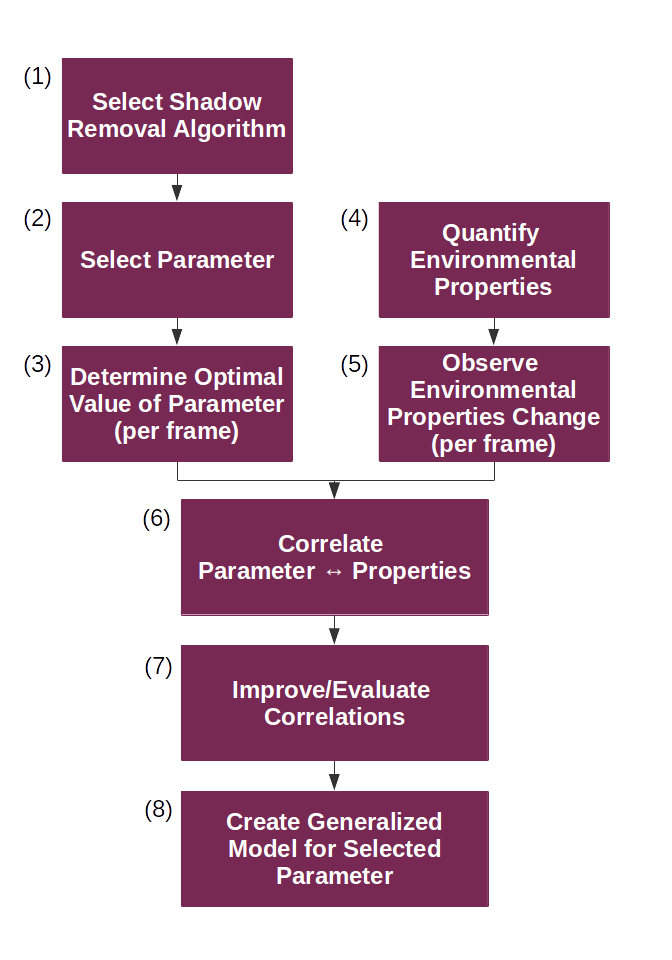
\includegraphics[width=.85\linewidth]{figures/background/overview.png}
%  \caption{Proof-of-concept overview.}
%  \label{fig:overview}
%\end{figure}

\begin{enumerate}
%\item \underline{Select Shadow Removal Algorithm}: The scope of the proof-of-concept model is restricted to one shadow removal algorithm. The algorithm selected must display reasonable sensitivity to both environmental changes. This proof-of-concept utilizes Physical shadow removal. Algorithm selection is detailed in section \ref{section:selectalgorithm}.

%\item \underline{Select Parameter}: In addition to demonstrating sensitivity to environmental change, the selected algorithm must also display sensitivity to parametric change. In section \ref{section:selectparameter}, we analyze multiple candidate parameters proven to significantly affect the accuracy of shadow removal.

\item \underline{Determine Optimal Value of Parameter (per frame)}: In accordance with our sensitivity analysis, each frame of a dataset has an optimal value for the selected parameter, i.e., there is an optimal value for which shadow removal is maximized. The process for extracting these optimal values is detailed in section \ref{section:datacollection}.

\item \underline{Quantify Environmental Properties}: Observed environmental properties are the most influential factor for creating an adaptive model. Section \ref{section:envassess} details identifying and quantifying salient environmental properties. 

%\item \underline{Observe Scene Properties Change (per frame)}: Our adaptive model requires that an algorithm may adapt to arbitrary environments as well as environmental changes. Environmental properties' values are recorded for each frame of a dataset.

\item \underline{Correlate Optimal Parameter Value and Environmental Properties}: For each dataset, optimal parameter values and environmental properties are recorded for each frame. By analyzing the correlation between the two sets, we receive a quantitative understanding of how well that environmental parameter would serve as the basis for an adaptive model. For example, if our optimal parameter value increases by $x\%$ from frame 1 to frame 2, and our environmental property also increases by $x\%$ from frame 1 to frame 2, that environmental property may be used to predict an appropriate value of our algorithm parameter. Consistent correlations are sought across each dataset to eliminate false positives.

\item \underline{Improve/Evaluate Correlations}: Many environmental properties exist that may not display direct correlation with a parameter's optimal value. We instead utilize these indirect properties as modulators to improve correlation observed with a primary environmental property. Multiple contributing environmental properties are combined to improve correlation and thereby shadow removal. Indirect properties are evaluated in sections \ref{section:nonlinearatten}, \ref{section:brightnessmodels}, and \ref{section:lowcSIFT}.

\item \underline{Create General Model for Selected Parameter}: Incorporating direct and indirect correlative environmental properties, we construct an adaptive model capable of calculating a new value for the algorithm parameter that improves shadow removal. This model is independent of dataset, and is calculated per frame, rather than applied to every frame in a dataset. Methodology for building this model is found in section \ref{section:model}.
\end{enumerate}

\end{document}

